\documentclass[11pt, a4paper]{article}
\linespread{1.5} 

\title{Comparing differences in citizen science and camera trap datasets in predicting habitat suitability for mammals in London}


\author{Uva Fung}
\date{%
    External supervisor: Dr. Chris Carbone -- Senior Research Fellow, Institute of Zoology, Zoological Society of London (chris.carbone@ioz.ac.uk)\\%
    Internal Supervisor: Professor Robert Ewers -- Professor of Ecology, Faculty of Natural Sciences, Department of Life Sciences (Silwood Park), Imperial College London (r.ewers@imperial.ac.uk)\\[2ex]%
}

\usepackage{lineno}
\usepackage{float}
\usepackage{indentfirst}
\usepackage[margin=2cm]{geometry}
\usepackage{graphicx}
\graphicspath{{}}


\begin{document}
  \maketitle
\newpage

\linenumbers

Keywords: Urban ecology, habitat suitability, citizen science, camera trapping, \textit{Erinaceus europaeus}, \textit{Vulpes vulpes}

\section{Introduction}
With increasing urban encroachment into natural environments, a growing number of wild animals are found in urban areas. An example is London, which is highly populated with over 8.9 million people but also home to multiple mammal species (ONS, 2020). To carry out successful conservation, it is vital to understand the distribution of species and their relationships with the anthropogenic environment. Such data are commonly collected via citizen science or camera traps. However, citizen science datasets only record presence but not absence data, and the observed species distribution are heavily biased towards easily accessible or highly populated areas (Guillera-Arroita et al., 2015). This potentially limits the accuracy of citizen science datasets. 

This study aims to answer two questions: i) What is the habitat suitability for native mammals in London? and, ii) What are the differences in habitat suitability predicted by citizen science and camera trap datasets? Building upon the work by Turner et al. (2021) on habitat suitability for London hedgehogs using citizen science data, I will model the habitat suitability for hedgehogs using camera trap data. The habitat suitability of foxes and badgers will also be modelled using both citizen science and camera trap datasets. I will then compare the resulting habitat suitability maps to determine if the two datasets predict different habitat suitability for each target mammal species. 


\section{Methods}

\underline{Step 1: Data collection} 

Camera trap and citizen science data are available as report form held by the Zoological Society London. Duplicate records with the same coordinates, year, and source dataset will be removed. To reduce sampling bias in citizen science data towards accessible or highly populated areas, I will only include records that have also reported sightings of other commonly seen mammals (Philips et al., 2009). The records will be used to indicate the presence or absence of target mammal species across London, divided into 100m x 100m grid squares. 
\vspace{\baselineskip}

\underline{Step 2: Model fitting and environmental predictions}

I will investigate how different environmental variables, such as garden, park, woodland, traffic volume, population and housing density affect the abundance of different target mammals. I will first investigate at what distance (100m, 250m, 500m, 750m, 1000m) would each environmental variable has the greatest influence on mammal abundance (Turner et al., 2021). This will be determined by fitting univariate binomial regression models in R and assessing the Area Under the Curve (AUC). For each environmental variable, the scale with the highest AUC will be used in subsequent analysis. Model fitting will be done using biomod2 package in R to determine the most parsimonious model in predicting mammal abundance, evaluated based on Akaike’s Information Criterion (AIC) (Thuiller et al., 2020). 
\vspace{\baselineskip}

\underline{Step 3: Habitat suitability map} 

Model fitting will provide an estimation of target mammal abundance based on the level of each environmental variable. I will use this data to construct a habitat suitability map using R, showing the relative habitat suitability of different areas in London. I will also determine the presence-absence threshold based on the threshold with the highest TSS value (Alejandro and Gerardo, 2015). The data will allow me to construct a binary map showing predictions of the presence or absence of different target mammals in London. 
\vspace{\baselineskip}

\underline{Step 4: Comparison between citizen science and camera trap datasets} 

The above processes will be repeated for each species using both citizen science data and camera data. The habitat suitability maps constructed will be compared for differences. 

\section{Anticipated output and outcomes}

This study will provide insights into how native mammals utilize different habitats. The maps generated will also provide an estimation of areas in London with high biodiversity, allowing more targeted conservation efforts on these important habitats. Comparison between results generated by citizen science and camera trap data will allow us to understand the merits and limitations of both data collection approaches, thereby improving future data collection. 

\section{Budget}
The total budget requested is £300.\\
Data storage: 1TB external SSD hard drive x2 (£115/each, total: £230)\\
Fieldwork: train tickets to Richmond and central London (Total: £70)


\begin{figure}[H]
  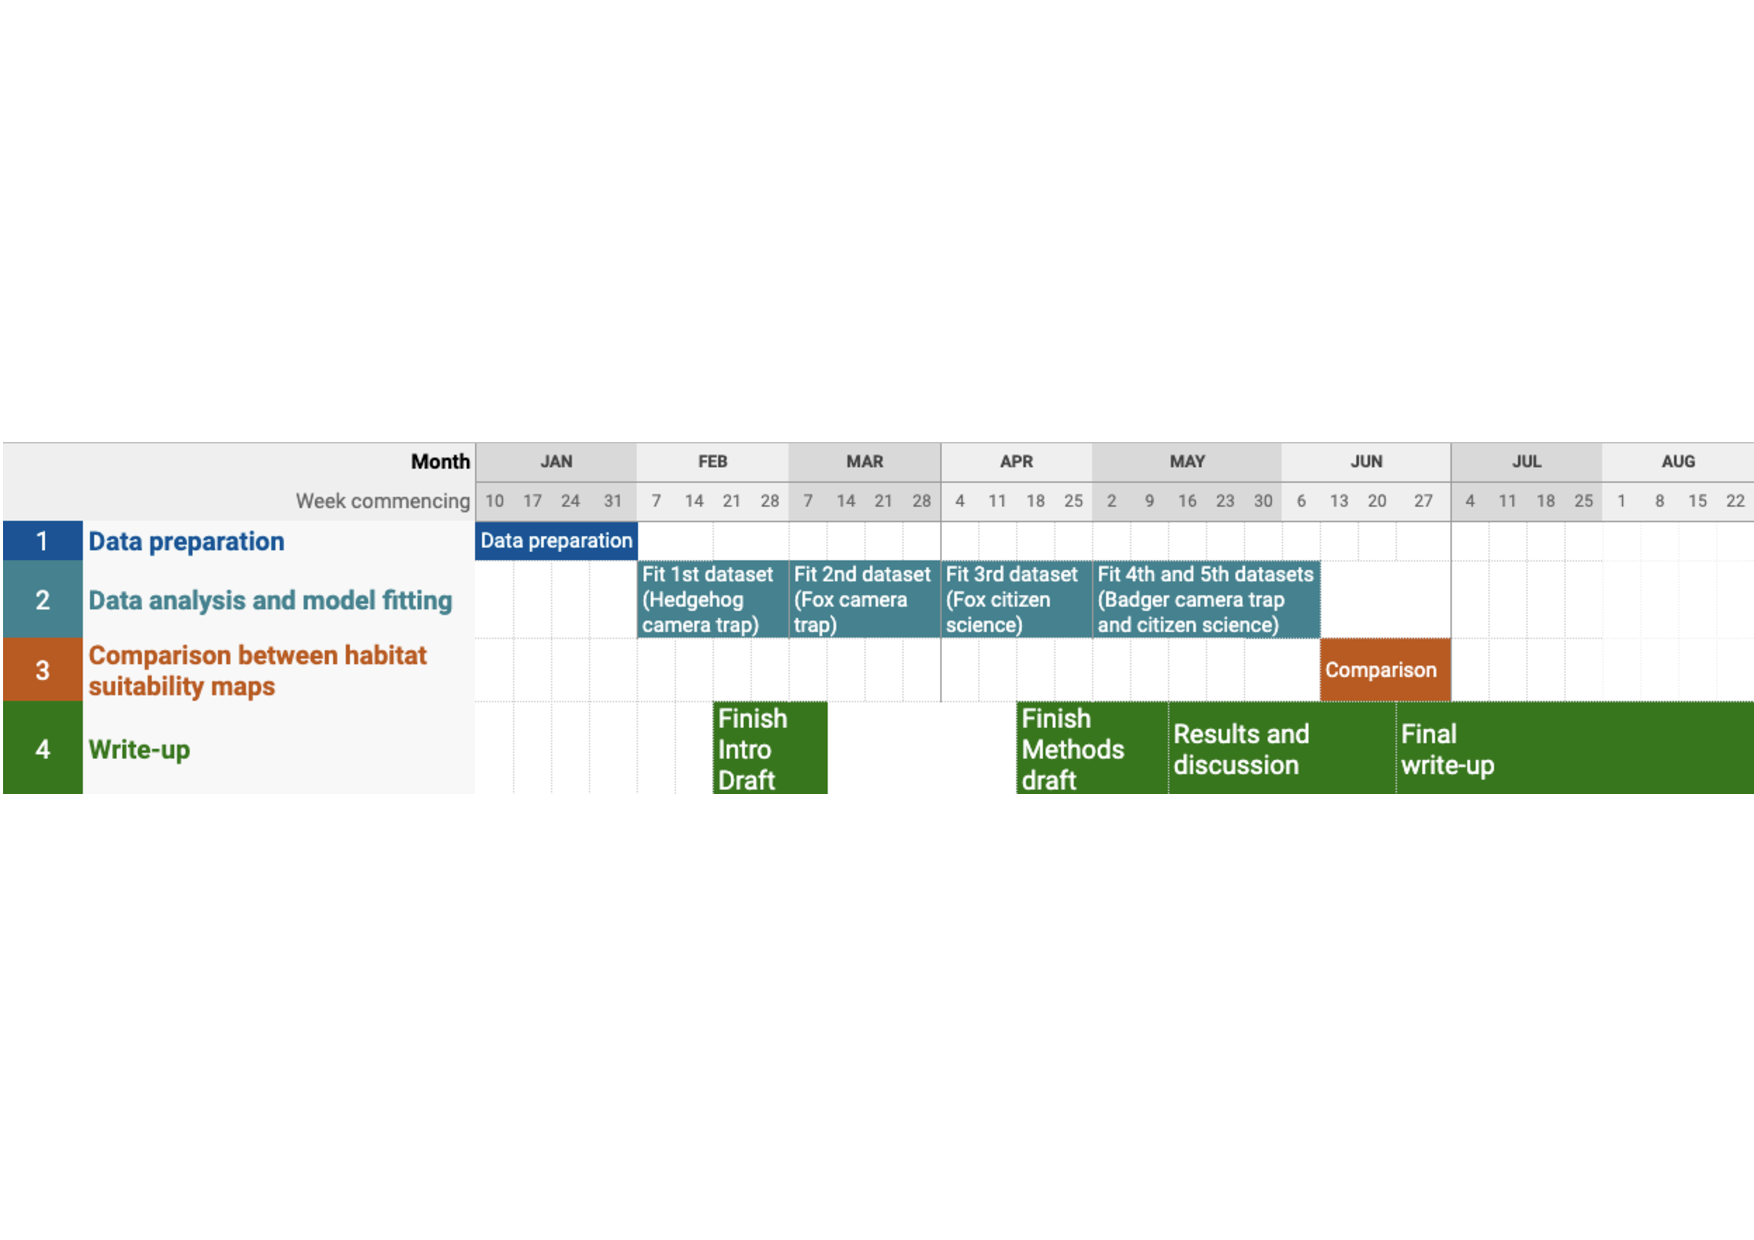
\includegraphics[width=\textwidth]{Gnatt_timeline.pdf}
\end{figure}

\newpage
\section{References}
Alejandro, R. and Gerardo, L. (2015). Goal-oriented evaluation of species distribution models’ accuracy and precision: True Skill Statistic profile and uncertainty maps. 10.7287/PEERJ.PREPRINTS.1208. 

Guillera-Arroita, G., Lahoz-Monfort, J.J., Elith, J., Gordon, A., Kujala, H., Lentini, P.E., McCarthy, M.A., Tingley, R. and Wintle, B.A. (2015). Is my species distribution model fit for purpose? Matching data and models to applications. Global Ecology and Biogeography, 24: 276–292.

Office for National Statistics (2020) Estimates of the population for the UK, England and Wales, Scotland and Northern Ireland: mid 2019.

Phillips, S.J., Dudik, M., Elith, J., Graham, C.H., Lehmann, A., Leathwick, J. and Ferrier, S. (2009). Sample selection bias and presence-only distribution models: implications for background and pseudo-absence data. Ecological Applications, 9: 181–197.

Thuiller, W., Georges, D., Engler, R. and Breiner, F. (2020). biomod2: Ensemble platform for species distribution modeling. R package version 3.4.6. https://CRAN.R-project.org/package=biomod2

Turner, J., Freeman, R. and Carbone, C. (2021). Using citizen science to understand and map habitat suitability for a synurbic mammal in an urban landscape: the hedgehog Erinaceus europaeus. Mammal Review. https://doi.org/10.1111/mam.12278


\newpage
I have seen and approved the proposal and the budget.

Professor Rob Ewers 20-Dec-2021
  
\includegraphics[width=0.5\textwidth]{RE_sign.pdf}
  
Dr. Chris Carbone 21-Dec-2021
  
\includegraphics[width=0.5\textwidth]{CC_sign.pdf}

\end{document}